\documentclass[tikz,border=4pt]{standalone}
\begin{document}
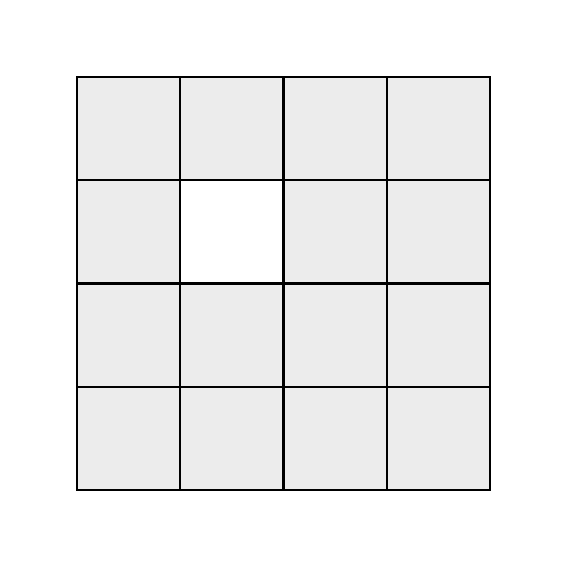
\begin{tikzpicture}[x=0.025cm,y=-0.025cm]
\path[use as bounding box] (0,0) rectangle (260,260);
\path[fill=gray!15,draw=black,line width=0.78pt] (25,25) rectangle (77.5,77.5);
\path[fill=gray!15,draw=black,line width=0.78pt] (77.5,25) rectangle (130,77.5);
\path[fill=gray!15,draw=black,line width=0.78pt] (130,25) rectangle (182.5,77.5);
\path[fill=gray!15,draw=black,line width=0.78pt] (182.5,25) rectangle (235,77.5);
\path[fill=gray!15,draw=black,line width=0.78pt] (25,77.5) rectangle (77.5,130);
\path[fill=gray!15,draw=black,line width=0.78pt] (130,77.5) rectangle (182.5,130);
\path[fill=gray!15,draw=black,line width=0.78pt] (182.5,77.5) rectangle (235,130);
\path[fill=gray!15,draw=black,line width=0.78pt] (25,130) rectangle (77.5,182.5);
\path[fill=gray!15,draw=black,line width=0.78pt] (77.5,130) rectangle (130,182.5);
\path[fill=gray!15,draw=black,line width=0.78pt] (130,130) rectangle (182.5,182.5);
\path[fill=gray!15,draw=black,line width=0.78pt] (182.5,130) rectangle (235,182.5);
\path[fill=gray!15,draw=black,line width=0.78pt] (25,182.5) rectangle (77.5,235);
\path[fill=gray!15,draw=black,line width=0.78pt] (77.5,182.5) rectangle (130,235);
\path[fill=gray!15,draw=black,line width=0.78pt] (130,182.5) rectangle (182.5,235);
\path[fill=gray!15,draw=black,line width=0.78pt] (182.5,182.5) rectangle (235,235);
\end{tikzpicture}
\end{document}
